\documentclass[border=2pt]{standalone}
\usepackage{lmodern}
\usepackage{tikz}
\usetikzlibrary{shapes.geometric, arrows, decorations.markings}
\usepackage{pgfplots}
\pgfplotsset{compat=1.10}
\makeatletter
\makeatother
\pgfplotsset{width=7cm,compat=1.12}




\begin{document}
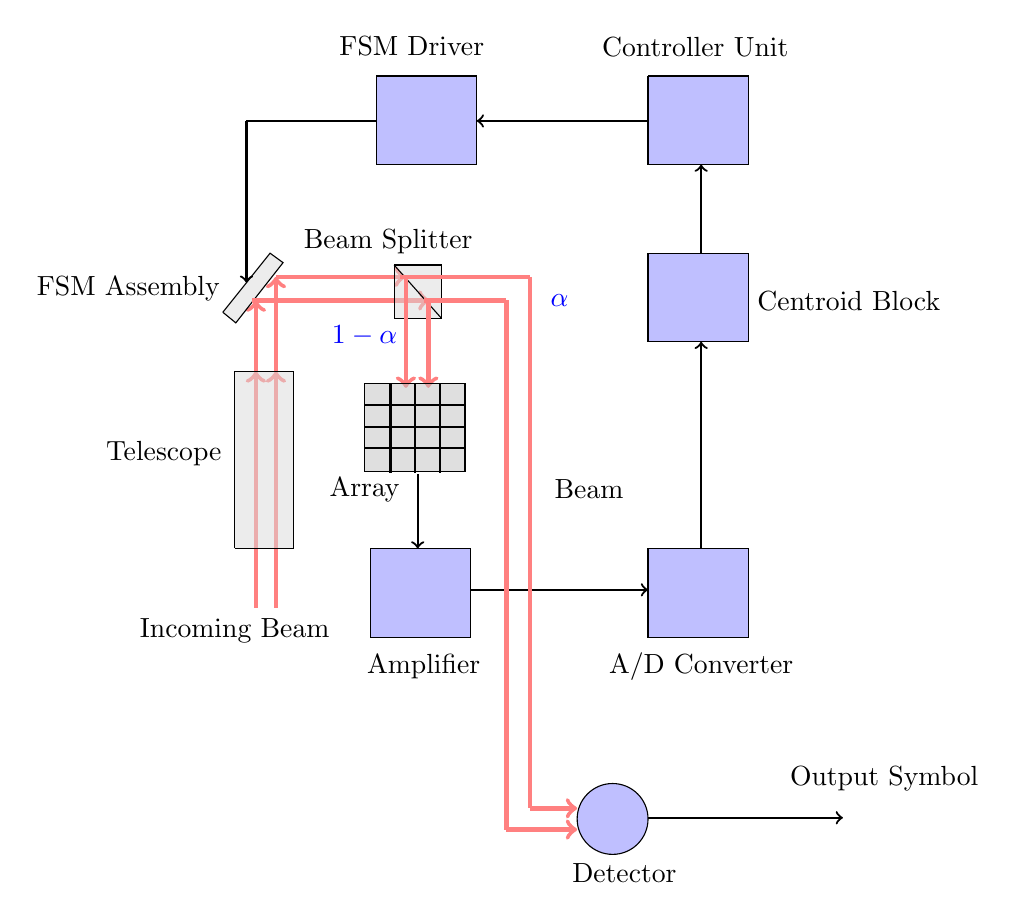
\begin{tikzpicture}[scale=1.5]

% Light into Telescope
\draw[->, ultra thick, color=red!50] (-0.32, -1)--(-0.32, 1);
\draw[->, ultra thick, color=red!50] (-0.15, -1)--(-0.15, 1);


% Telescope
\draw[-, fill=gray!30, fill opacity = 0.5] (-0.5, -0.5)--(-0.5, 1)--(0, 1)--(0,-0.5)--(-0.5, -0.5);

% Light into of FSM
\draw[->, ultra thick, color=red!50] (-0.32, 1)--(-0.32, 1.6);
\draw[->, ultra thick, color=red!50] (-0.15, 1)--(-0.15, 1.8);

% FSM
\draw[-, fill=gray!30, fill opacity = 0.5] (-0.6, 1.5)--(-0.2, 2)--(-0.09, 1.92)--(-0.49, 1.41)--(-0.6, 1.5);

% Light into Beam Splitter
\draw[->, ultra thick, color=red!50] (-0.35, 1.6)--(1.15, 1.6);
\draw[->, ultra thick, color=red!50](-0.15, 1.8)--(0.95, 1.8);

% Beam Splitter
\draw[-, fill=gray!30, fill opacity=0.5] (0.85, 1.9)--(1.25, 1.9)--(1.25, 1.45)--(0.85, 1.45)--(0.85, 1.9);
\draw[-] (0.85, 1.9)--(1.25, 1.45);

% Light into Array of Detectors
\draw[->, ultra thick, color=red!50] (0.95, 1.8)--(0.95, 0.86);
\draw[->, ultra thick, color=red!50] (1.14, 1.59)--(1.14, 0.86);

% Array of Detectors
\begin{scope}[shift={(-1.1, 3.9)}, scale=1.0]
\draw[-, fill=gray!50, fill opacity=0.5](1.7, -3)--(2.55, -3)--(2.55, -3.75)--(1.7, -3.75)--(1.7, -3);
\draw[-, thick](1.7, -3.185)--(2.55, -3.185);
\draw[-, thick](1.7, -3.37)--(2.55, -3.37);
\draw[-, thick](1.7, -3.55)--(2.55, -3.55);
\draw[-, thick](2.13, -3)--(2.13, -3.76);
\draw[-, thick](1.92, -3)--(1.92, -3.76);
\draw[-, thick](2.34, -3)--(2.34, -3.76);
\end{scope}

% Amplifier
\draw[->, thick] (1.05, 0.13)--(1.05, -0.5);
\draw[-, fill=blue!50, fill opacity=0.5](0.65, -0.5)--(1.5, -0.5)--(1.5, -1.25)--(0.65, -1.25)--(0.65, -0.5);

% A/D Converter
\draw[->, thick] (1.5, -0.85)--(3, -0.85);
\draw[-, fill=blue!50, fill opacity=0.5](3, -0.5)--(3.85, -0.5)--(3.85, -1.25)--(3, -1.25)--(3, -0.5);

% Position Measurement
\draw[->, thick] (3.45, -0.5)--(3.45, 1.25);
\draw[-, fill=blue!50, fill opacity=0.5](3, 2)--(3.85, 2)--(3.85, 1.25)--(3, 1.25)--(3, 2);



% Controller
\draw[->, thick] (3.45, 2)--(3.45, 2.75);
\draw[-, fill=blue!50, fill opacity=0.5](3, 3.5)--(3.85, 3.5)--(3.85, 2.75)--(3, 2.75)--(3, 3.5);

% FSM Driver
\draw[->, thick] (3.0, 3.12)--(1.55, 3.12);
\draw[-, fill=blue!50, fill opacity=0.5](0.7, 3.5)--(1.55, 3.5)--(1.55, 2.75)--(0.7, 2.75)--(0.7, 3.5);
\draw[-, thick] (0.7, 3.12)--(-0.4, 3.12);
\draw[->, thick] (-0.4, 3.12)--(-0.4, 1.75);

% Light into Beam Splitter 1
\draw[-, ultra thick, color=red!50] (1.1, 1.6)--(1.8, 1.6);
\draw[-, ultra thick, color=red!50](0.9, 1.8)--(2.0, 1.8);
\draw[-, ultra thick, color=red!50] (1.8, 1.6)--(1.8, -2.88);
\draw[-, ultra thick, color=red!50](2.0, 1.8)--(2.0, -2.70);
% Light out of Beam Splitter 1
\draw[->, ultra thick, red!50](2.0, -2.70)--(2.4, -2.70);
\draw[->, ultra thick, red!50](1.8, -2.88)--(2.4, -2.88);


% Symbol Detector
\begin{scope}[shift={(1.65,-3.23)}]
\draw[ fill=blue!50, fill opacity = 0.5] (1.05, 0.44) circle (0.3 cm);

% Output of Symbol Detector
\draw[->, thick](1.35, 0.45)--(3, 0.45);

\end{scope}
















\node at (3.45, -1.5) {  A/D Converter};

\node at (1.1, -1.5) {  Amplifier};

\node at (0.6, 0) {  Array};

\node at (4.7, 1.6) {  Centroid Block};


\node at (3.4, 3.75) {  Controller Unit};

\node at (1.0, 3.75) { FSM Driver};

\node at (-1.1, 0.3) {  Telescope};

\node at (-1.4, 1.7) {  FSM Assembly};

\node at (0.8, 2.1) {  Beam Splitter};

\node at (-0.5, -1.2) {  Incoming Beam};

\node at (2.25, 1.6){\textcolor{blue}{$\alpha$}};

\node at (0.6, 1.3){\textcolor{blue}{$1-\alpha$}};

\node at (2.8, -3.25){  Detector};




\node at (2.5, 0){  Beam};

\node at (5, -2.45){ Output Symbol};



% \node at (6.3, -6.35){ \begin{tabular}{l} \large Data Fusion \\ \large (MRC or EGC) \end{tabular}};






\end{tikzpicture}


\end{document}